
\documentclass{article}

% Language setting
% Replace `english' with, e.g., `spanish' to change the document language
\usepackage[english]{babel}

% Set page size and margins
% Replace `letterpaper' with `a4paper' for UK/EU standard size
\usepackage[letterpaper,top=2cm,bottom=2cm,left=3cm,right=3cm,marginparwidth=1.75cm]{geometry}

% Useful packages
\usepackage{amsmath}
\usepackage{graphicx}
\usepackage{relsize}
\usepackage[colorlinks=true, allcolors=blue]{hyperref}
\usepackage{tikz}
\usetikzlibrary{shapes,arrows,positioning}
\usepackage{float} % Include the float package in your preamble

\title{Monte Carlo Localization for Autonomous Vehicle Navigation}
\author{HAzMAT (Team 12)}

\begin{document}
\maketitle



\section{Introduction: Alonso}

Localization is a vital problem within the field of robotics. For an autonomous robot to navigate through an environment, whether known or unknown, it must reliably know its pose. Within the framework of RSS, localization combines signal processing and geometric perception to create a geometric world model that is useful for motion planning. The lab builds upon previous labs by moving beyond the naivety of unquestioningly following walls or cones. It gives the robot an added layer of information through a relative location. In combination with Lab 6, this lab is a crucial component to autonomous navigation through a city, which will be implemented in the Final Challenge. 

Monte Carlo Localization requires two processes running in parallel: updating the robots pose estimate with odometry data (motion model), and then re-initializing the estimates of the robot pose given the likelihood of observed LiDAR scans (sensor model). This section will briefly explain the reasoning behind the processes, but further detail can be found in the Technical Approach section. Given a set of guesses about the pose of the car, to accurately follow the robot's trajectory, they must be updated for the car's movement. The odometry data is given in a local frame, which must be converted to the global frame to accurately place the robot within the map. Not every guess for the robot's pose is good, which is why the sensor model is critical. Using a set of predetermined parameters, the sensor model will scan through every pose guess, compare every observed LiDAR scan to the expected scan, and return a likelihood that the pose guess accurately represents the robot's location. Based upon the likelihoods, pose estimates are resampled (using a numpy library). The ultimate idea is that given enough points and time for the resampling, the pose estimates will converge, and the average of these poses will accurately represent the true robot pose.



\section{Technical Approach}



\subsection{Motion Model: Alonso, Thomas}

The motion model is designed to accurately update the robot's pose as it moves through its environment. The implementation works by updating poses through odometry messages. The ultimate goal of the motion model is to implement it into the particle filter to continuously reflect the robot pose estimates, updated for the observed motion of the robot.  

The first step in the motion model is to calculate the odometry data in terms of dx, dy, and dtheta vectors. These vectors are obtained by creating a custom function that utilizes a time step, the linear velocity in x and y, and the angular velocity in z. The velocities are integrated with respect to time, dt, to obtain dx, dy, and dtheta. 

The next step of the motion model is the implementation of noise. The noise is meant to simulate error and also spreads out pose estimates so they are more likely to capture the robot's true pose if the initial guess is suboptimal. A function to implement Gaussian noise as a vector was created, which allowed the creation of custom noise for each particle in the dataset. The following distributions were used for each element of the pose:

\[
x: \mathcal{N}(\mu = 0.0, \sigma^2 = 0.1 \text{ m})
\]
\[
y: \mathcal{N}(\mu = 0.0, \sigma^2 = 0.1 \text{ m})
\]
\[
\theta: \mathcal{N}(\mu = 0.0, \sigma^2 = 0.01 \text{ rad})
\]

A Gaussian distribution centered around 0 was utilized due to a lack of systematic error. While the x and y variances should theoretically be different due to the physical dependence on x motion to produce y motion in a car, the same value for simplicity and efficacy. Finally, the variance of $\theta$ is an order of magnitude smaller since its units are radians, not meters. All the variances produce noise of the same order of magnitude as the expected motion (velocity of ~2m/s) during a time step of 1/20 to 1/50 of a second. It made physical sense to keep these orders of magnitude related to allow for a reasonable amount of spreading but still allowing for rapid convergence.

Finally, the noise vector was combined with the vector of the dx, dy, and dtheta vectors, fed as inputs to the function, and updated (noisy) dx, dy, and dtheta vectors were obtained. These values were then fed into the final step of the implementation to update the poses. Due to frame differences between the global pose and local odometry data, the global pose update relies on the following set of equations, which are derived from Euler angles:

\begin{align*}
    x_{\text{new,map}} &= x_{\text{old,map}} + \cos(\theta_{\text{old,map}}) \times \Delta x_{\text{observed,local}} - \sin(\theta_{\text{old,map}}) \times \Delta y_{\text{observed,local}} \\
    y_{\text{new,map}} &= y_{\text{old,map}} + \sin(\theta_{\text{old,map}}) \times \Delta x_{\text{observed,local}} + \sin(\theta_{\text{old,map}}) \times \Delta y_{\text{observed,local}} \\
    \theta_{\text{new,map}} &= \theta_{\text{old,map}} + \Delta \theta_{\text{observed,local}}
\end{align*}

The impact that the change in \(\Delta \theta\) would have on \(x_{\text{new,map}}\) and \(y_{\text{new,map}}\) was neglected because the time steps in the odometry are 1/20 to 1/50 of a second which is small enough that a linear approximation is more than adequate. This is especially true due to the eventual resampling of points, eliminating the compounding error in pure odometry integration.

Ultimately, each particle was updated, and the particle matrix was returned as the motion model's evaluation function output. These values were aligned with the sample test cases and allowed for the efficient implementation of this step into the overall system. The figure below summarizes the steps in the motion model. 
\vspace{1cm}

\begin{figure}[htbp]
    \centering
    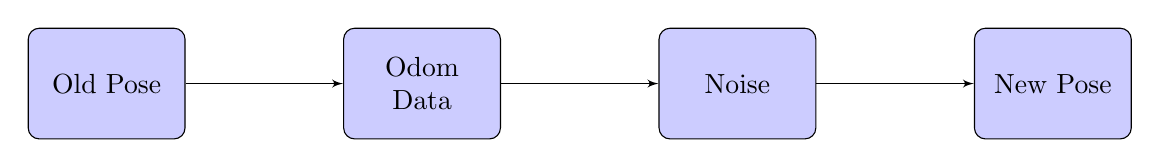
\begin{tikzpicture}[node distance=2cm, auto]
        % Define block styles
        \tikzstyle{block} = [rectangle, draw, fill=blue!20, text width=5em, text centered, rounded corners, minimum height=4em]
        \tikzstyle{line} = [draw, -latex']

        % Nodes
        \node [block] (Old_Pose) {Old Pose};
        \node [block, right=2cm of Old_Pose] (Odom_Data) {Odom Data};
        \node [block, right=2cm of Odom_Data] (Noise) {Noise};
        \node [block, right=2cm of Noise] (New_Pose) {New Pose};

        % Arrows
        \path [line] (Old_Pose.east) -- (Odom_Data.west);
        \path [line] (Odom_Data.east) -- (Noise.west);
        \path [line] (Noise.east) -- (New_Pose.west);
    \end{tikzpicture}
    \caption{Flowchart illustrating Motion Model}
    \label{fig:flowchart}
\end{figure}

\subsection{Sensor Model: Thomas}
The sensor model is another critical component enabling the robot to gather information about its location within the environment. The implementation utilizes LiDAR sensor data and a probabilistic approach to evaluate the likelihood of the robot's pose based on the laser scan observations. 

At a high level, attempting to calculate the probability of every particle at every time step is highly computationally expensive, requiring not only iterating through a near-infinite, continuous distribution of points but also calculating the probabilities for each point. The problem is discretized by introducing a 200 by 200 grid of points to simplify the calculation at each time step, significantly minimizing the number of particles. A lookup table was also created, providing the ability to pre-compute the probability data given initial conditions, look up new particles at the following time steps, and update their associated probabilities. 

To model the sensor behavior, a 200 by 200 2D array was created that contains the probability distribution for each sensor's measurements, given the true distance to obstacles. This table is first pre-computed based on given parameters, including the likelihood of various error weighting parameters as well as the standard deviation of the distribution. The formulas used for the probability model calculation are shown below. 
$$
p_{\text{hit}}(x) = 
\begin{cases} 
\eta\frac{1}{\sqrt{2\pi\sigma^2}}\text{exp}^\left(-\frac{(z_k^{(i)}-d)^2}{2\sigma^2}\right) & \text{if } 0 \leq z_k \leq z_{max}  \\
0 & \text{otherwise}
\end{cases}
$$
$$
p_{\text{short}}(x) = 
\begin{cases} 
\frac{2}{d_{\text{val}}} \left(1 - \frac{x}{d_{\text{val}}}\right) & \text{if } 0 \leq x \leq d_{\text{val}} \text{ and } d_{\text{val}} \neq 0 \\
0 & \text{otherwise}
\end{cases}
$$
$$
p_{\text{max}}(x) = 
\begin{cases} 
\frac{1}{\epsilon} & \text{if } z_{\text{max}} - \epsilon \leq x \leq z_{\text{max}} \\
0 & \text{otherwise}
\end{cases}
$$
$$
p_{\text{rand}}(x) = 
\begin{cases} 
\frac{1}{z_{\text{max}}} & \text{if } 0 \leq x \leq z_{\text{max}} \\
0 & \text{otherwise}
\end{cases}
$$
$$
p_z = \alpha_{\text{short}} \cdot p_{\text{short}}(z_{\text{val}}) + \alpha_{\text{max}} \cdot p_{\text{max}}(z_{\text{val}}) + \alpha_{\text{rand}} \cdot p_{\text{rand}}(z_{\text{val}})
$$

The table is indexed at runtime by discretizing the measurements and the computed ranges. Finally, it is normalized to ensure that the entire span of probabilities adds up to 1. 

Notably, this precomputed calculation does $p_{hit}$ separately. The first idea was to compute $p_z$ at once for each grid point; however, this was a harder computational problem than computing $p_{hit}$ individually for each particle. This allows the normalization of the $p_{hit}$ values to be done independently of the rest of the table easily. After this, the rest of $p_z$ was applied to each grid point with a final normalization applied for each grid point.

Next, a simulated laser scan was created using the PyScanSimulator2D class and ray tracing was performed from the poses. This generates a matrix of simulated laser values and compares them to the actual LiDAR readings. The sensor model ultimately functions by retrieving the likelihood of each particle's pose given the observation by indexing into the table with the discretized LiDAR measurements and simulated ranges, then multiplying the probabilities across all beams for each particle. 

Finally, the sensor model also recognizes the map from the ROS topic, converting it into a numpy array and setting up the simulated laser scan data in the context of this map. This is what allows the model to utilize ray tracing in a known environment the robot must navigate. 

In summary, the sensor model uses a precomputed, discretized table in order to optimize probability calculations. It interprets laser scan data in the context of the map for an efficient localization algorithm. 


\vspace{1cm}
\begin{figure}[htbp]
  \centering
  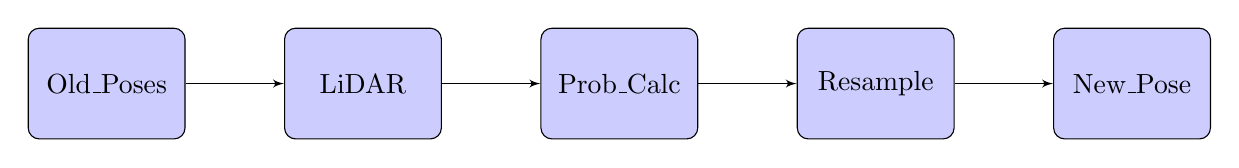
\begin{tikzpicture}[node distance=1.0cm, auto]
    % Define block styles
    \tikzstyle{block} = [rectangle, draw, fill=blue!20, text width=5.0em, text centered, rounded corners, minimum height=4.0em]
    \tikzstyle{line} = [draw, -latex']

    % Nodes
    \node [block] (Old_Poses) {Old\_Poses};
    \node [block, right=1.25cm of Old_Poses] (LiDAR) {LiDAR};
    \node [block, right=1.25cm of LiDAR] (Probability_Calc) {Prob\_Calc};
    \node [block, right=1.25cm of Probability_Calc] (Resample) {Resample};
    \node [block, right=1.25cm of Resample] (New_Pose) {New\_Pose};  

    % Arrows
    \path [line] (Old_Poses.east) -- (LiDAR.west);
    \path [line] (LiDAR.east) -- (Probability_Calc.west);
    \path [line] (Probability_Calc.east) -- (Resample.west);
    \path [line] (Resample.east) -- (New_Pose.west);  

  \end{tikzpicture}
  \caption{Scaled-down Flowchart illustrating Sensor Model}
  \label{fig:scaled_flowchart_sensor_model}
\end{figure}



\subsection{Particle Filter: Heath}
Once the motion and sensor models were working, assembly and construction of the complete Monte Carlo Localization algorithm was next.  \par
Before the algorithm starts, particle initialization must be done. The particles were initialized around a clicked location in Rviz, using the 2D Pose Estimate button which was published as a PoseWithCovarianceStamped message. The point's position was obtained from the message and used its quaternion to compute its theta angle. To create a randomly distributed cloud of particles around the clicked point, uniform noise was added to the clicked point position, $(x_{\text{point}}, y_{\text{point}})$. For the yaw angle of the particles, while initial estimations started with uniform noise with a range of $2\pi$, concentrating the particle yaw angles around the robot yaw angle was found to yield much better performance. \par
\begin{align*}
x_{\text{part}} &= x_{\text{point}} + U(-1, 1) &
y_{\text{part}} &= y_{\text{point}} + U(-1, 1) &
\theta_{\text{part}} &= \mathcal{N}(\theta_{\text{point}}, 0.1^{2})
\end{align*}
Once the particles were initialized, sensor data and odometry data begin to be collected. In brevity, the algorithm will update the particles positions every time odometry data is received while also computing the particle probabilities and resampling them every time sensor data is received. These two actions are separated in two different callbacks as the rate at which this data is collected is different. Refer to \textbf{Figure 3} for a step-by-step breakdown of all the processes within the particle filter.\par

\tikzstyle{block} = [rectangle, draw, text width=3cm, text centered, rounded corners, minimum height=1cm]
\tikzstyle{line} = [draw, -latex']

\begin{figure}[htbp]
    \centering
    \resizebox{15cm}{!}{
    \begin{tikzpicture}[node distance = 0.75cm, auto, every node/.style={align=center}]
    % Place nodes
    \node [block, text width=4cm, minimum height=1cm] (click) {Click Point in Rviz};
    \node [block, below=of click, text width=4cm, minimum height=1cm] (initialize) {Initialize Particles};
    \node [block, below left=of initialize, text width=3.5cm] (odometry) {Obtain \\ Odometry Message};
    \node [block, below right=of initialize, text width=3.5cm, minimum height=1cm] (laser) {Receive \\ LaserScan Data};
    \node [block, below=of odometry, text width=4cm, minimum height=1cm] (compute) {Convert Message \\ to Data};
    \node [block, below=of laser, text width=4cm, minimum height=1cm] (sensor) {Compute Probabilities with Sensor Model};
    \node [block, below=of compute, text width=4cm, minimum height=1cm] (update) {Update Particles with Motion Model};
    \node [block, below=of sensor, text width=4cm, minimum height=1cm] (resample) {Resample Particles};
    \node [block, below right=of update, text width=4cm, minimum height=1cm] (average) {Calculate \\ Average Particle};
    \node [block, below=of average, text width=4cm, minimum height=1cm] (transform) {Publish Transform \\ to TF Tree};
    
    % Draw edges
    \path [line] (click) -- (initialize);
    \path [line] (initialize.west) -| (odometry);
    \path [line] (initialize.east) -| (laser);
    \path [line] (odometry) -- (compute);
    \path [line] (laser) -- (sensor);
    \path [line] (compute) -- (update);
    \path [line] (sensor) -- (resample);
    \path [line] (update) |- (average.west);
    \path [line] (resample) |- (average.east);
    \path [line] (average) -- (transform);
    \end{tikzpicture}
    }
    \caption{Full overview of the processes within the particle filter. Everytime there is '2D Pose Estimate' within Rviz, a new set of particles are initialized. Then the left side of the chart shows the operations included in the odometry callback function and the right side showcases the operations included in the laser callback function. Once each callback obtains it's new set of particles, they are always averaged and the new expected robot pose is published to the TF tree.}
    \label{fig:flowchart}
\end{figure}


\subsubsection{Odometry Callback}
The odometry callback function receives odometry information as an Odometry message which must be converted before fed into the motion model. Within the Odometry message is a TwistWithCovariance message that contains the cars linear and angular velocity which can be integrated over time to calculate the odometry data.
\begin{align*}
    \Delta x &= \int_{t_0}^{t_1} u \, dt &
    \Delta y &= \int_{t_0}^{t_1} v \, dt &
    \Delta \theta &= \int_{t_0}^{t_1} \omega_{z} \, dt 
\end{align*}
The motion model is then used to update the current particles with recently calculated odometry data (information on this calculation can be found in \textbf{Section 2.2}). Once the new particle locations are computed, they are averaged to find the new estimated robot pose. 

\subsubsection{Laser Callback}
The laser callback function received a LaserScan message which contains the LiDAR data collected from the car. The sensor model is called to calculate the probabilities for each particle which are used during the resampling process. Before resampling can occur the probability vector is normalized to ensure it sums to 1.
\begin{equation*}
    \text{Normalized Probabilities} = \frac{\text{Probabilities}}{\sum_{i=1}^{n} p_{i}}
\end{equation*}
To resample the particles, indices were selected from the range of number of particles, given the normalized probabilities, and ensured replacement of selected indices so that those with higher probability could be picked more than once.
\begin{equation*}
    \text{Selected Indices} : \text{Multinominal}(n,p=\text{Normalized Probabilities}, replace=\text{True})    
\end{equation*}
The generated indices were then used to define a new batch of particles to be averaged and published.

\subsubsection{Compute Average and Publish Transform}
Once the callback functions generated their new set of particles, they must be averaged to find the new expected robot pose. For the robot position this just entails a simple linear average where $(x_i, y_i)$ are the particle locations and $n$ is the number of particles.
\begin{align*}
    x_{\text{new}} &= \frac{\sum_{i=1}^{n} x_i}{n} &
    y_{\text{new}} &= \frac{\sum_{i=1}^{n} y_i}{n}
\end{align*}
For the theta values, a circular mean was utilized.
\begin{align*}
    x_{\theta_{\text{avg}}} &= \frac{\sum_{i=1}^{n} \cos{\theta_{i}}}{n} &
    y_{\theta_{\text{avg}}} &= \frac{\sum_{i=1}^{n} \sin{\theta_{i}}}{n}
\end{align*}
The mean of the coordinates was converted back into an angle.
\begin{equation*}
    \theta_{\text{new}} = \arctan\left(\frac{y_{\theta_{\text{avg}}}}{x_{\theta_{\text{avg}}}}\right)
\end{equation*}
Now the expected robot pose is output given the updated particles which represents the transform between the map frame and the base link (or car frame).
\begin{equation*}
    \mathlarger{T}_{\text{map}}^{\text{base\_link}} = [x_{\text{new}}, y_{\text{new}}, \theta_{\text{new}}]
\end{equation*}
This transform must be published to the TF tree so that the next time odometry data is collected, the robot knows the frame the data is published within.


\section{Particle Filter Experimental Evaluation}

\subsection{Motion Model: Alex}
To test that the motion model functioned properly, a comparison of the pose estimate generated from the Monte Carlo Localization algorithm's odometry to the ground truth odometry produced by \textit{base link} was used. Initially, the unit tests passed; however, upon integration with the sensor model, major issues were encountered such as the particles propagating in the opposite direction as the initial pose. The next step was individually testing the motion model first, as it is responsible for determining the poses of the particles. 

The model was tested qualitatively and quantitatively. RViz allowed easy visual testing through PoseArray messages overlayed with odometry pose estimate as an Odometry message. 

The two figures below show a qualitative test ran on the particle filter with only the motion model active. Figure 1 was taken 1 second after initialization, while Figure 2 was taken 4 seconds after initialization. These tests verified the expected behavior as the poses are spreading out (due to noise) but are still centered around the car, verifying the odometry.

\begin{figure}[H]
    \centering
    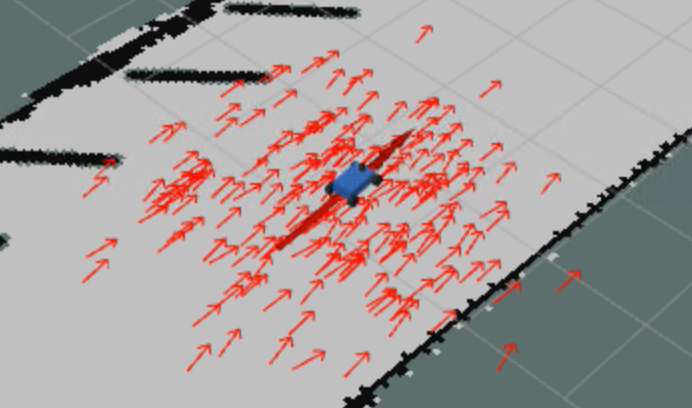
\includegraphics[width=0.8\textwidth]{1 sec.png} % Replace 'example-image' with your image filename
    \caption{Motion Model poses 1 second after initialization. The darker red, longer arrows display the average particle pose estimate. In this frame it is visually right on the robot's origin.}
    \label{fig:1sec}
\end{figure}

\begin{figure}[H]
    \centering
    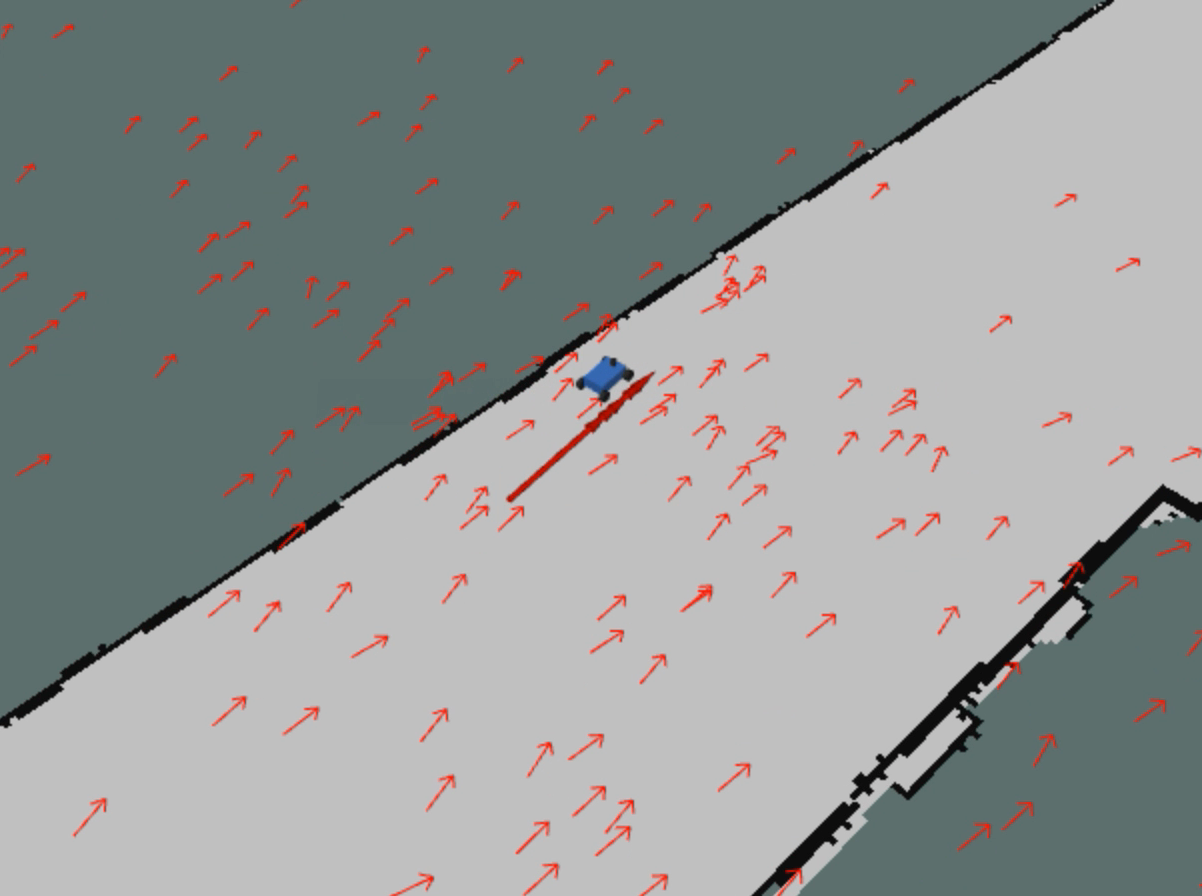
\includegraphics[width=0.8\textwidth]{20secs.png} % Replace 'example-image' with your image filename
    \caption{Motion Model poses 20 seconds after initialization. This shows how the pose estimate (shown in darker red, longer arrows) diverged from the robot's origin.}
    \label{fig:20sec}
\end{figure}

On the quantitative side, Pythagorean distance was used to evaluate the model: 
\begin{equation}
d = \sqrt{(x_{truth}-x_{est})^2+(y_{truth}-y_{est})^2}
\end{equation}
Due to the nature of the motion model, the particles' relative distance will increase, which causes the average particle pose estimate to slowly diverge from ground truth. Therefore, it is expected that $d$ will increase as time increases. The figure below corroborates the expected behavior:

\begin{figure}[H]
    \centering
    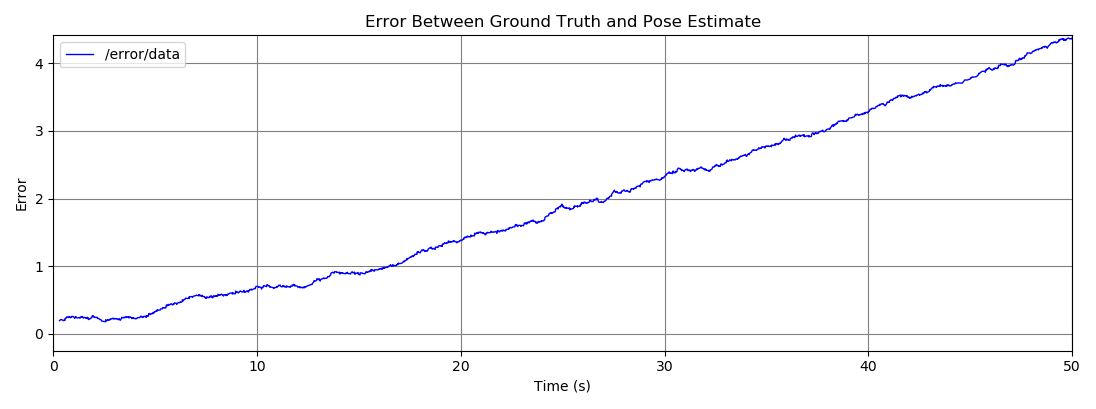
\includegraphics[width=0.8\textwidth]{error_motion_model.png}
    \caption{Error between the ground truth odometry and the the pose estimate. As expected, the error increases with time because the particles spread out due to noise in motion model. }
    \label{fig:motion_model_err}
\end{figure}

In the subsequent section on the particle filter, a similar metric was used to test the integration of the motion and sensor models to evaluate the accuracy of the estimate.

\subsection{Sensor Model: Alex}
The sensor model is imperative for the successful localization of the robot over time. The issue of the filter converging onto the wall was eventually fixed after lots of testing and assistance from TA's. Knowing that the motion model was confidently functional after the testing delineated previously, the next step was testing the sensor model. Due to the nature of particle filters, if the sensor model's probability distribution is very accurate, i.e. it produces high-probability, narrow peaks, it counter-intuitively will be less reliable because of the addition of noise onto the particles. This minute perturbation shifts the particles' $x$ and $y$ coordinates, and since the probability distribution houses narrow peaks, the altered particles are more likely to land on a wider peak, even if it may be less probable. Let 
\begin{align*}
    p &= \begin{bmatrix}
           p_{1} \\
           p_{2} \\
           \vdots \\
           p_{200}
         \end{bmatrix}
\end{align*}
be the probability distribution of the particles represented as a column vector of the probability of each particle. In this case, 200 particles were selected to compute our pose estimates.
The following figure shows the difference between the pre-computed $p$ with a squashed version, i.e. $p^{\frac{1}{3}}$.

\begin{figure}[H]
    \centering
    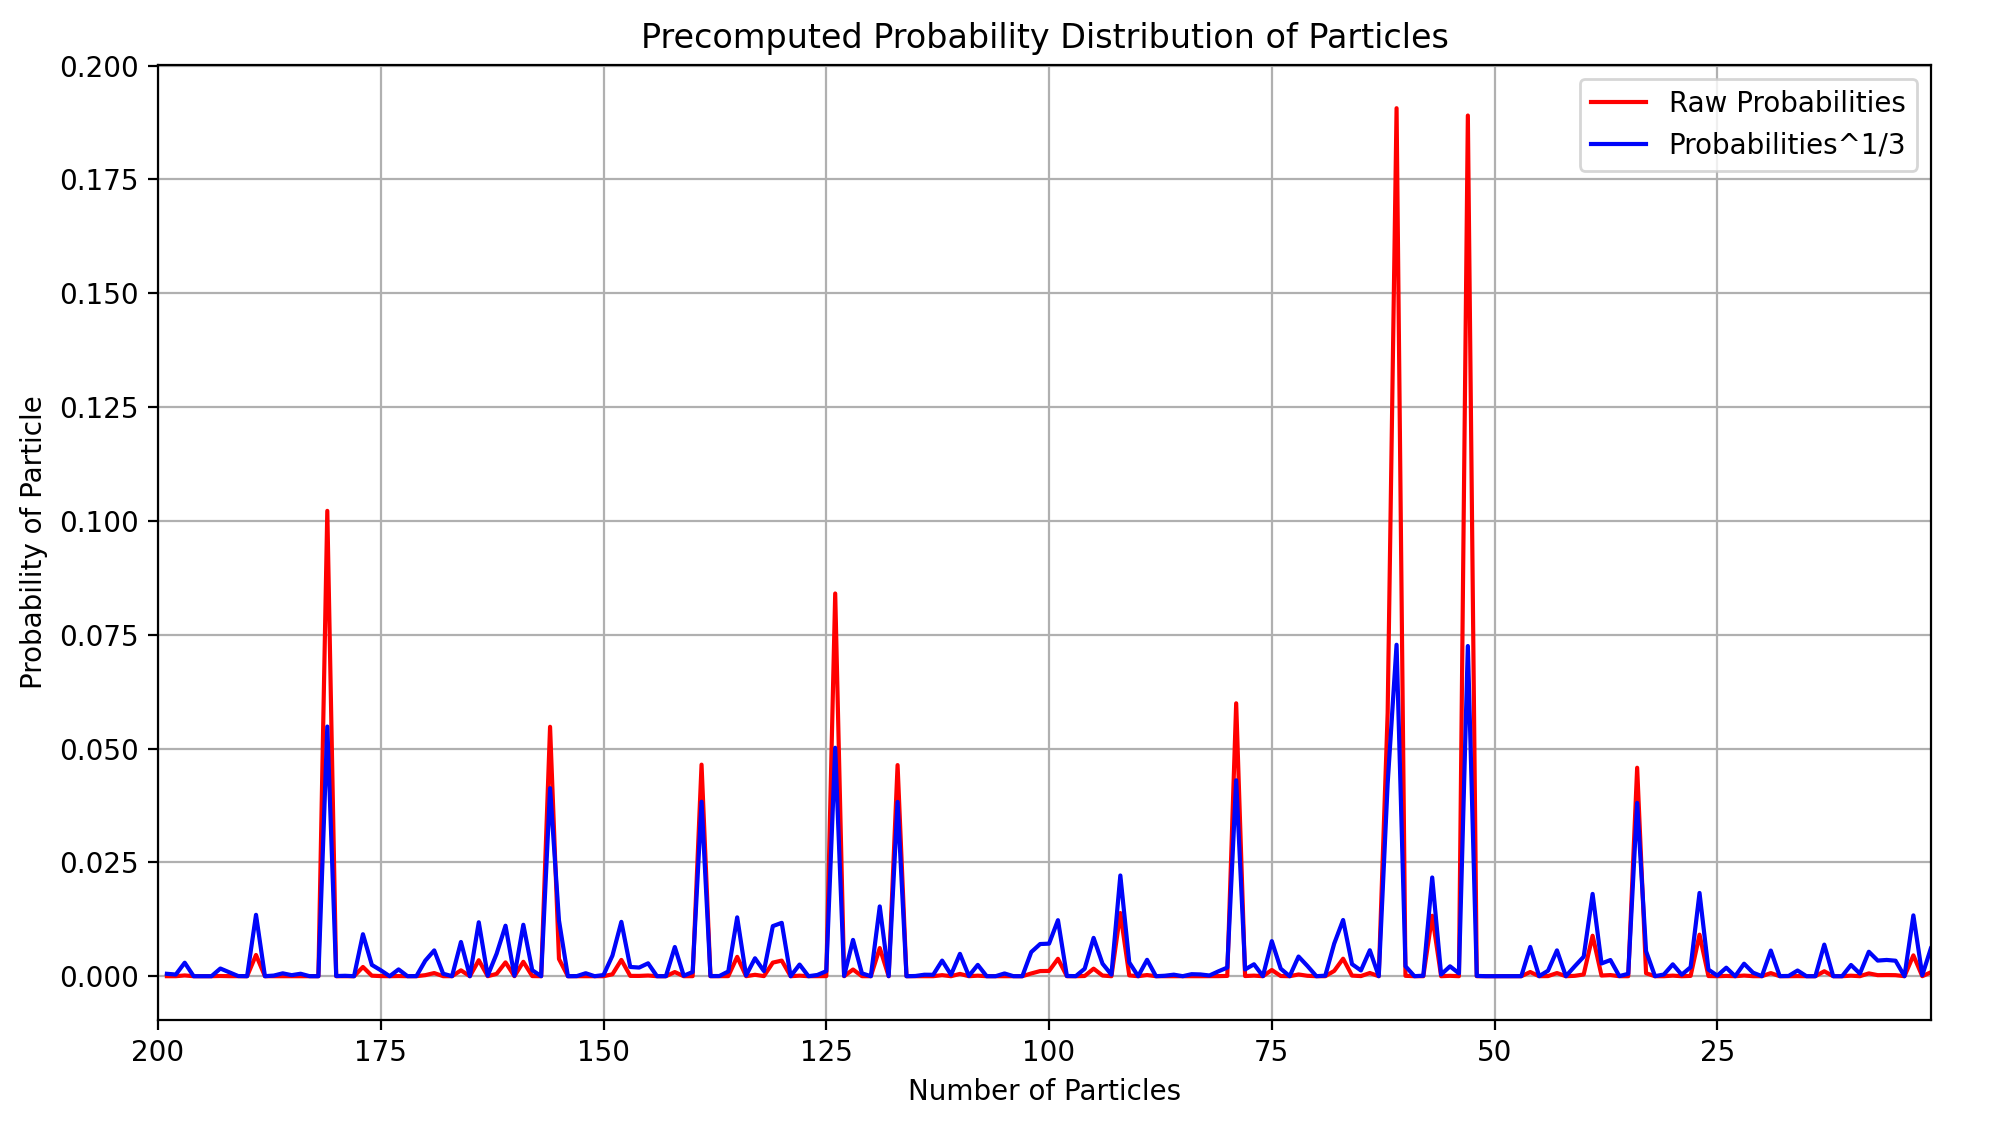
\includegraphics[width=0.8\textwidth]{prob.png} % Replace 'example-image' with your image filename
    \caption{Probability distribution $p$ overlayed with $p^{\frac{1}{3}}$. This shows the tall, narrow peaks of $p$ and the wider, shorter peaks of $p^{\frac{1}{3}}$.}
    \label{fig:probabilities}
\end{figure}

 $p^{\frac{1}{3}}$ exhibits much shorter peaks, but they are wider, as the minute peaks bordering the much more probable ones increased in probability. This is the desired behavior, as now, with an functional motion model, there will no longer be an issue with converging to the wrong peak. This will be shown by the tests on the fully integrated particle filter, described subsequently.
\subsection{Particle Filter: Marcelo}
In a functional particle filter, all of the particles converge on or around the robot's current location with respect to world, and these must have a high probability of being correct. To quantify these measure, the average distance from the true position and the probability's standard deviation are utilized.

Average distance from the current position serves as a metric on whether the particles can find the correct location for the robot. This is computed by finding the average position of all particles, then comparing it in simulation to the current position.
\begin{align}
    dist_{avg} &= (1-\frac{x_{avg}}{x_{current}}) + (1-\frac{y_{avg}}{y_{current}})
\end{align}

This results in the following graph:
\begin{figure}[H]
    \centering
    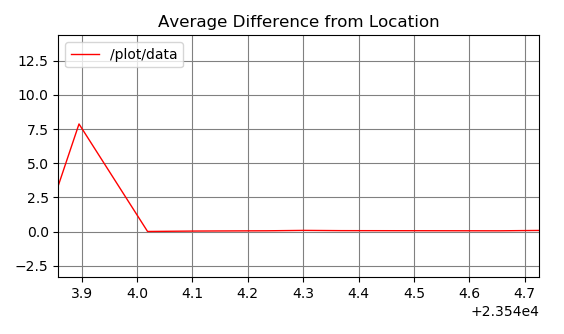
\includegraphics[width=0.8\textwidth]{avg_dist.png}
    \caption{Average Distance Error}
    \label{fig:avg-dist}
\end{figure}
In the figure there is a large initial spike from randomized starting positions, and then the error decreases to 0, meaning that the average position is the same as the actual location.

The probability standard deviation is used to see how spread out the particle probabilities from the mean. This shows that particles must be close to each other.

This results in the following:
\begin{figure}[H]
    \centering
    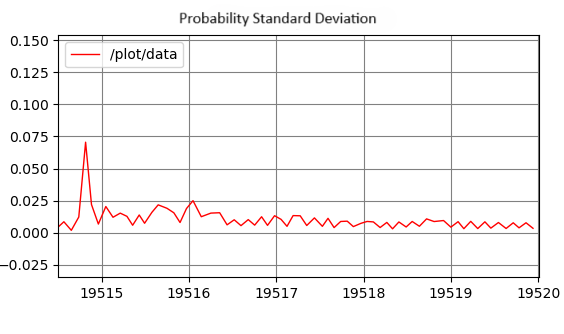
\includegraphics[width=0.8\textwidth]{prob_std_dev.png}
    \caption{Probability Standard Deviation}
    \label{fig:prob-std-dev}
\end{figure}
Again, a larger initial spike is observed due to the randomized initial values, which decrease as the standard deviation approaches zero, which means that the confidence on the correct position is higher.

With both of these, a high level of confidence is obtained on where the particles are located, as well as that the average position is accurate. 


\section{Conclusion: Alonso}

This lab culminated in the successful development and implementation of a Monte Carlo Localization algorithm within simulation. Each piece works individually, as well as jointly, to initialize particles, update positions, down sample LiDAR scans, calculate probabilities, and then resample particles. While the code is successful in tracking the robot's pose within simulation, it has yet to achieve the same results on a physical robot. The culprit for this deficiency comes down to the myriad of issues in getting the code to properly run, which unfortunately did not leave enough time to finalize the implementation on the physical robot. Moving from simulation to physical robot is no small task as there are different parameters and coordinate conventions. Particularly for the final challenge ensuring accurate performance on the robot will be critical. 

As for simulation, other potential areas for improvement include fine tuning noise parameters, down sampling rates, as well the number of particles initialized.



\section{Lessons Learned}

\subsection{Alonso}

This lab was full of teaching moments. Technically, I was able to further develop my programming and algorithmic skills. This lab forced me to go back through lectures as I thought through the implementation of the Monte Carlo Localization algorithm. Several of my assumptions about the algorithm were wrong, such as how resampling worked, so it was very enlightening to correct myself. From a communications standpoint, this lab was the first lab which featured a report. I believe that through writing this lab, my technical writing has improved, particularly due to advice from the CI staff. I have a better understanding of how to weave findings and figures into a technical piece. Finally, from a teamwork standpoint, this lab was also enriching. One lesson that I have taken away is that we need to start even earlier (and we had started very early already). The challenges encountered while debugging and dividing the labor during the editing process were very valuable learning experiences. Overall, a very difficult, but rewarding lab.

\subsection{Heath}
The big takeaway from this lab was code modularization. With an algorithm as complicated at Monte Carlo Localization, there are many different tasks and functions. If these aren't properly separated and tested, finding errors within the full integration of the algorithm is near impossible. At the start of the lab, we had all of our code within our callback functions which increased the difficulty of finding bugs. After reevaluating the necessary calculations within each step of our particle filter, we wrote specific methods for each task that could be individually unit tested to ensure correctness. The other main area of learning during this lab was utilizing Rviz and rqt graph for visualization and graphing of key metrics. Without obtaining and understanding for the current status of the particles or probabilities is was extremely difficult to find errors.

\subsection{Alex}
In the end, after finding the smallest bug causing the entire algorithm to fail (thanks to the TAs), it hit me how important it is to organize code. Thankfully, most of us realized this and modularized several functions within the larger scoped callbacks. This allowed for us to test different steps of the Monte Carlo localization algorithm and made the debugging process easier. As the time I poured into the lab increased, I felt a lot more familiar with the steps and how each one fed into the next, building the full localization of the robot. This was incredibly gratifying. From the communication side, I realized how important it is to communicate clearly with the team. Due to the convoluted nature of this lab, it was imperative that the work I was doing was shared with the rest of the team, so that there was no extra work nor inefficiency occurring. With all of us working on different parts of the code, I needed to be able to fully understand my contributions to sensor model so that I could confidently explain it to the people working on motion model when it came to integration. Additionally, I learned from previous labs that it is okay and encouraged for me to ask for help early, and I felt that I improved on that this time around, as I was able to ask for help, both from TAs in office hours and from my teammates. Lastly, I am very grateful for our CI instructor Jane, as the Zoom meeting we had with her, albeit it being one hour only, was incredibly helpful in guiding me with writing this report and to keep improving on my presentation skills.

\subsection{Thomas}\
My biggest takeaway from this lab is to approach problems modularly. We had spent days scanning through the code, searching for which of our many functions and models was the culprit of the algorithm's failure, whether it be non-convergence, movement in a wrong or random direction, or improperly converging to walls. These problems took days to solve, but their cause was a few lines scattered throughout various modules. Going forward, it is important to validate each module independently through simulation to diagnose bugs early on before large-scale implementation, even if the test cases seemingly pass. I also really valued our team's conversation with Jane, our CI instructor, who gave us tips on making a better-formatted presentation and building our public speaking skills. Her removing "um" lesson has stuck with me, and I implemented tactics during the briefing she taught us. I also gained an appreciation for our team's ability to work on tasks in parallel, with Alonso and Heath taking on the motion model and Marcelo, Alex, and I working on the sensor model, but then later assisting in correcting bugs throughout both models and their communication with each other. I personally found it difficult at first to understand the logic behind the motion model, but after discussing it with my team over Discord, I was able to help debug and identify issues in otherwise foreign code. 

\subsection{Marcelo}
The main lesson I got from this is that developing systems is a continuous process, even when any given part seems complete. The clearest example of this was when designing particle filter, since the particles wouldn't converge on the car. It turned out to be an error in the sensor model, which had previously passed test cases. As such, we need to make sure that we don't take any part as completed, even when it seems to be working perfectly. Another key lesson is time management, especially starting tasks early as to allow for unexpected delays or longer than usual turnarounds.



\bibliographystyle{alpha}
\bibliography{sample}

[MIT-RSS24] MIT-RSS, "Visual\_servoing," GitHub, 2024. [Online]. Available: https://github.com/mit-rss/visual\_servoing.
\vspace{0.5cm}
[PioneeringMinds19] Pioneering Minds, "We’re Being Sold A Fantasy About Self-Driving Cars," Pioneering Minds, 26-Jul-2019. Available: https://www.pioneeringminds.com/were-being-sold-a-fantasy-about-self-driving-cars/.


\end{document}